\subsection{On Premise Edge}

Among the 
%distinct application scenarios of 
different flavors of the edge computing paradigm, one addresses the needs of real-time and/or data-intensive applications with on premise infrastructure deployments. Examples range from the Industry 4.0, also known as IoT 4.0, to
%Similarly, edge computing is also seen as an enabling technology towards 
smart homes and offices~\cite{Porambage:2018}. For these scenarios, edge infrastructure may consist of domestic gateways, single-board computers, or even full scale servers.

%Differently from the outsourcing model popularized by cloud computing, 
On premise resources are generally acquired and deployed to cope with the requirements from specific applications whose demand is known beforehand. Still, an efficient and automated management of these resources is needed to render solutions economic. As the technology evolves, the adoption of a serverless architecture empowered by the FaaS model becomes attractive for private deployments. This is even more true for the scenarios in which the demand for services is expected to change (e.g., following the daily changes of a smart factory). 

%\begin{figure}[tpb]
%	\centering
%	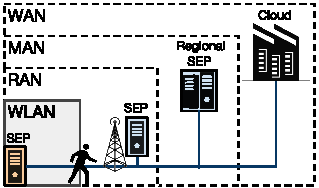
\includegraphics[width=1\linewidth]{Figs/Edge_Cloud_Continuum}
%	\caption{Different types of edge infrastructure forming a computing continuum; applications hosted by IoT and mobile devices switch between on premise and on demand SEPs hosting similar functions.}
%	\label{fig:Edge_Cloud_Continuum}
%\end{figure}

On premise and on demand SEPs may also form a computing continuum that allows mobile applications empowered with self-managing capabilities~\cite{OrsiniBL16,Baresi:2018} to make use of the best available resources at each context. The characteristics of the FaaS model --- stateless and granular functions independently deployed --- facilitates the realization of such a continuum by allowing the seamless switching between on premise accessible through private WLAN to on demand SEPs accessible through RAN. %Figure~\ref{fig:Edge_Cloud_Continuum} illustrates the aforementioned scenario. 


%As an example, let us think of a smart home environment. Users make use of a browser-based editor to specify automation workflows composed of sensors, functions, and actuators. Sensors data are published to specific topics of the Publish-Subscribe Service, triggering the activation of functions responsible for the analysis of data and generation of actuation commands. 

%and the provisioning and allocation of resources should benefit from the automation of FaaS tools.



%The FaaS model was originally conceived as an alternative execution model for cloud computing. 


%In this sense, the advantages characterizing the FaaS model may be exploited in the materialization of on premise edge computing.




%For this, on premise SEPs should exhibit the computational resources and services (discussed along the present section) compatible with targeted applications. Also, on premise and on demand SEPs can form an infrastructure continuum supporting mobility.

%We conclude the present section with a typical smart home scenario in which a plethora of sensors providehttps://www.overleaf.com/project/5bb1f5b57d8ebf292d2436ed information about the environment and actuators operate on different equipment. Communication with the domestic SEP is performed with lightweight protocols (e.g., COAP~\cite{} and MQTT~\cite{}). Functions are triggered by events (e.g., from sensors), direct calls (e.g., from smart devices) or execution flows (e.g., from a microclimate analysis workflow). Figure~\ref{} illustartes this scenario.
